% 注意事项:编译两次,以确保目录、页码完整显示

\def\allfiles{}

\documentclass[14pt,a4paper,UTF8,twoside]{article}

% Formatting Packages ——————————————————————————————————————
\usepackage{multicol}
\usepackage{multirow}
\usepackage{enumitem}
\usepackage{indentfirst}
\usepackage[toc]{multitoc}

% Math & Physics Packages ————————————————————————————
\usepackage{amsmath, amsthm, amsfonts, amssymb}
\usepackage{setspace}
\usepackage{physics}
\usepackage{cancel}
\usepackage{nicefrac}
\usepackage{unicode-math} % 允许数学公式使用特定字体

% Image-related Packages —————————————————————————————
\usepackage{float} % 浮动体环境
\usepackage{subcaption} % 子图包
\usepackage{graphics, graphicx}
\usepackage{tikz, tikz-qtree}
\usetikzlibrary{arrows.meta}
\usepackage{pgfplots}
\pgfplotsset{compat=1.18}
\usepackage{xcolor}
\usepackage{fourier-orns}
\usepackage{lipsum}

% Colour Palette ——————————————————————————————————————
\definecolor{merah}{HTML}{F4564E}
\definecolor{merahtua}{HTML}{89313E}
\definecolor{biru}{HTML}{60BBE5}
\definecolor{birutua}{HTML}{412F66}
\definecolor{hijau}{HTML}{59CC78}
\definecolor{hijautua}{HTML}{366D5B}
\definecolor{kuning}{HTML}{FFD56B}
\definecolor{jingga}{HTML}{FBA15F}
\definecolor{ungu}{HTML}{8C5FBF}
\definecolor{lavender}{HTML}{CBA5E8}
\definecolor{merjamb}{HTML}{FFB6E0}
\definecolor{mygray}{HTML}{E6E6E6}
\definecolor{mygreen}{rgb}{0,0.6,0}
\definecolor{mymauve}{rgb}{0.58,0,0.82}

% Theorems ————————————————————————————————————————————
\usepackage{tcolorbox}
\usepackage{changepage}
\tcbuselibrary{skins,breakable,theorems}

\newcounter{hitung}
\setcounter{hitung}{\thesection}

\makeatletter
	% Proof 证明如下
	\def\tcb@theo@widetitle#1#2#3{\hbox to \textwidth{\textsc{\large#1}\normalsize\space#3\hfil(#2)}}
	\tcbset{
		theorem style/theorem wide name and number/.code={ \let\tcb@theo@title=\tcb@theo@widetitle},
		proofbox/.style={skin=enhancedmiddle,breakable,parbox=false,boxrule=0mm,
			check odd page, toggle left and right, colframe=black!20!white!92!hijau,
			leftrule=8pt, rightrule=0mm, boxsep=0mm,arc=0mm, outer arc=0mm,
			left=3mm,right=3mm,top=0mm,bottom=0mm, toptitle=0mm,
			bottomtitle=0mm,colback=gray!3!white!98!biru, before skip=8pt, after skip=8pt,
			before={\par\vskip-2pt},after={\par\smallbreak},
		},
	}
	\newtcolorbox{ProofBox}{proofbox}
	\makeatother
	
	\let\realproof\proof
	\let\realendproof\endproof
	\renewenvironment{proof}[1][Prove:]{\ProofBox\strut\textsc{#1}\space}{\endProofBox}
        \AtEndEnvironment{proof}{\null\hfill$\blacksquare$}
        % Definition 定义环境
	\newtcbtheorem[use counter=hitung, number within=section]{dfn}{定义}
	{theorem style=theorem wide name and number,breakable,enhanced,arc=3.5mm,outer arc=3.5mm,
		boxrule=0pt,toprule=1pt,leftrule=0pt,bottomrule=1pt, rightrule=0pt,left=0.2cm,right=0.2cm,
		titlerule=0.5em,toptitle=0.1cm,bottomtitle=-0.1cm,top=0.2cm,
		colframe=white!10!biru,
		colback=white!90!biru,
		coltitle=white,
		shadow={1.3mm}{-1.3mm}{0mm}{gray!50!white}, % 添加阴影
        coltext=birutua!60!gray, title style={white!10!biru}, rbefoe skip=8pt, after skip=8pt,
		fonttitle=\bfseries,fontupper=\normalsize}{dfn}

	% 答题卡
	\newtcbtheorem[use counter=hitung, number within=section]{ans}{解答}
	{theorem style=theorem wide name and number,breakable,enhanced,arc=3.5mm,outer arc=3.5mm,
		boxrule=0pt,toprule=1pt,leftrule=0pt,bottomrule=1pt, rightrule=0pt,left=0.2cm,right=0.2cm,
		titlerule=0.5em,toptitle=0.1cm,bottomtitle=-0.1cm,top=0.2cm,
		colframe=white!10!biru,
		colback=white!90!biru,
		coltitle=white,
		shadow={1.3mm}{-1.3mm}{0mm}{gray!50!white}, % 添加阴影
        coltext=birutua!60!gray, title style={white!10!biru}, before skip=8pt, after skip=8pt,
		fonttitle=\bfseries,fontupper=\normalsize}{ans}

	% Axiom
	\newtcbtheorem[use counter=hitung, number within=section]{axm}{公理}
	{theorem style=theorem wide name and number,breakable,enhanced,arc=3.5mm,outer arc=3.5mm,
		boxrule=0pt,toprule=1pt,leftrule=0pt,bottomrule=1pt, rightrule=0pt,left=0.2cm,right=0.2cm,
		titlerule=0.5em,toptitle=0.1cm,bottomtitle=-0.1cm,top=0.2cm,
		colframe=white!10!biru,colback=white!90!biru,coltitle=white,
		shadow={1.3mm}{-1.3mm}{0mm}{gray!50!white!90}, % 添加阴影
        coltext=birutua!60!gray,title style={white!10!biru},before skip=8pt, after skip=8pt,
		fonttitle=\bfseries,fontupper=\normalsize}{axm}
 
	% Theorem
	\newtcbtheorem[use counter=hitung, number within=section]{thm}{定理}
	{theorem style=theorem wide name and number,breakable,enhanced,arc=3.5mm,outer arc=3.5mm,
		boxrule=0pt,toprule=1pt,leftrule=0pt,bottomrule=1pt, rightrule=0pt,left=0.2cm,right=0.2cm,
		titlerule=0.5em,toptitle=0.1cm,bottomtitle=-0.1cm,top=0.2cm,
		colframe=white!10!merah,colback=white!75!pink,coltitle=white, coltext=merahtua!80!merah,
		shadow={1.3mm}{-1.3mm}{0mm}{gray!50!white!90}, % 添加阴影
		title style={white!10!merah}, before skip=8pt, after skip=8pt,
		fonttitle=\bfseries,fontupper=\normalsize}{thm}
	
	% Proposition
	\newtcbtheorem[use counter=hitung, number within=section]{prp}{命题}
	{theorem style=theorem wide name and number,breakable,enhanced,arc=3.5mm,outer arc=3.5mm,
		boxrule=0pt,toprule=1pt,leftrule=0pt,bottomrule=1pt, rightrule=0pt,left=0.2cm,right=0.2cm,
		titlerule=0.5em,toptitle=0.1cm,bottomtitle=-0.1cm,top=0.2cm,
		colframe=white!10!hijau,colback=white!90!hijau,coltitle=white, coltext=hijautua!80!brown,
		shadow={1.3mm}{-1.3mm}{0mm}{gray!50!white}, % 添加阴影
		title style={white!10!hijau}, before skip=8pt, after skip=8pt,
		fonttitle=\bfseries,fontupper=\normalsize}{prp}


	% Example
	\newtcolorbox[use counter=hitung, number within=section]{cth}[1][]{breakable,
		colframe=white!10!jingga, coltitle=white!90!jingga, colback=white!85!jingga, coltext=black!10!brown!50!jingga, colbacktitle=white!10!jingga, enhanced, fonttitle=\bfseries,fontupper=\normalsize, attach boxed title to top left={yshift=-2mm}, before skip=8pt, after skip=8pt,
		title=Contoh~\thetcbcounter \ \ #1}

	% Catatan/Note
	\newtcolorbox{ctt}[1][]{enhanced, 
		left=4.1mm, borderline west={8pt}{0pt}{white!10!kuning}, 
		before skip=6pt, after skip=6pt, 
		colback=white!85!kuning, colframe= white!85!kuning, coltitle=orange!60!kuning!25!brown, coltext=orange!60!kuning!25!brown,
		fonttitle=\bfseries,fontupper=\normalsize, before skip=8pt, after skip=8pt,
		title=\underline{Catatan}  #1}
	
	% Komentar/Remark
	\newtcolorbox{rmr}[1][]{
		,arc=0mm,outer arc=0mm,
		boxrule=0pt,toprule=1pt,leftrule=0pt,bottomrule=5pt, rightrule=0pt,left=0.2cm,right=0.2cm,
		titlerule=0.5em,toptitle=0.1cm,bottomtitle=-0.1cm,top=0.2cm,
		colframe=white!10!kuning,colback=white!85!kuning,coltitle=white, coltext=orange!60!kuning,
		fonttitle=\bfseries,fontupper=\normalsize, before skip=8pt, after skip=8pt,
		title=Komentar  #1}

\usepackage{booktabs} % 表格库
\usepackage{titlesec} % 标题库
\usepackage{fancyhdr} % 页眉页脚库
\usepackage[sorting=none]{biblatex}
\usepackage{array}
\addbibresource{references.bib} % 指定你的.bib文件名称

\date{} % 留空,以让编译时去除日期

%———————————————注意事项—————————————————%

% 1、如果编译显示失败,但没有错误信息,就是 filename.pdf 正在被占用
% 2、在文件夹中的终端使用 Windows > xelatex filename.tex 也可编译

%—————————————华东师范大学———————————————%

% 论文制作时须加页眉,页眉从中文摘要开始至论文末
% 偶数页码内容为:华东师范大学硕士学位论文,奇数页码内容为学位论文题目

%————————定义 \section 的标题样式————————%

% 注意:\chapter 等命令,内部使用的是 \thispagestyle{plain} 的排版格式
% 若需要自己加上页眉,实际是在用 \thispagestyle{fancy} 的排版格式
% 加上下面这一段指令,就能够让 \section 也使用 fancy 的排版格式
% 本质就是让目录、第一页也能够显示页眉、页脚

\fancypagestyle{plain}{
  \pagestyle{fancy}
}

\title{华东师范大学软件学院课程作业} % 模板
\titleformat{\section}
    {\normalfont\bfseries\Large} % 字体大小、字体系列(\bfseries 为加粗)
    {\thesection}{1em}{}

% ———————————设置章节的中文格式———————————%
\renewcommand\thesection{\chinese{section} \hspace{0pt}}
\renewcommand\thesubsection{\arabic{subsection} \hspace{0pt}}
% \renewcommand\thesubsubsection{\alph{subsubsection} \hspace{0pt}} % 字母编号
% \hspace{0pt} 是为了确保在章节编号和章节题目之间不要有空格,使得排版更为美观
    
%—————————————页面基础设置———————————————%

\usepackage{geometry}
\geometry{left=10mm, right=10mm, top=20mm, bottom=20mm}

%————————————设置页眉、页脚——————————————%

\pagestyle{fancy} % 设置 plain style 的属性

% 设置页眉

\fancyhead[RE]{\leftmark} % Right Even 偶数页右侧显示章名 \leftmark 最高级别章名
\fancyhead[LO]{\rightmark} % Left Odd 奇数页左侧显示节名 \rightmark 第二级别节名
\fancyhead[C]{华东师范大学软件学院课程作业} % Center 居中显示
\fancyhead[LE,RO]{~\thepage~} % 在偶数页的左侧,奇数页的右侧显示页码
\renewcommand{\headrulewidth}{1.2pt} % 页眉与正文之间的水平线粗细

% 设置页脚:在每页的右下脚以斜体显示书名

\fancyfoot[RO,RE]{\it Lab Report By \LaTeX} % 使用意大利斜体显示
\renewcommand{\footrulewidth}{0.5pt} % 页脚水平线宽度

%——————设置页码:在底部居中显示页码———————%

\usepackage{lastpage} % 页码数库
\pagestyle{fancy}
\fancyfoot[C]{\kaishu 第 \thepage 页 \ 共 \pageref{LastPage} 页} % LastPage 需要二次编译以获取总页数

%——————————————代码块设置———————————————%

\usepackage{listings} % 代码块包
\lstset {
    backgroundcolor=\color{white},   % choose the background color; you must add \usepackage{color} or \usepackage{xcolor}
    basicstyle=\footnotesize,        % the size of the fonts that are used for the code
    breakatwhitespace=false,         % sets if automatic breaks should only happen at whitespace
    breaklines=true,                 % sets automatic line breaking
    captionpos=bl,                   % sets the caption-position to bottom
    commentstyle=\color{mygreen},    % comment style
    deletekeywords={...},            % if you want to delete keywords from the given language
    escapeinside={\%*}{*},           % if you want to add LaTeX within your code
    extendedchars=true,              % lets you use non-ASCII characters; for 8-bits encodings only, does not work with UTF-8
    frame=single,                    % adds a frame around the code
    keepspaces=true,                 % keeps spaces in text, useful for keeping indentation of code (possibly needs columns=flexible)
    keywordstyle=\color{blue},       % keyword style
    % language=Python,               % the language of the code
    morekeywords={*,...},            % if you want to add more keywords to the set
    numbers=left,                    % where to put the line-numbers; possible values are (none, left, right)
    numbersep=5pt,                   % how far the line-numbers are from the code
    numberstyle=\tiny\color{mygray}, % the style that is used for the line-numbers
    rulecolor=\color{black},         % if not set, the frame-color may be changed on line-breaks within not-black text (e.g. comments (green here))
    showspaces=false,                % show spaces everywhere adding particular underscores; it overrides 'showstringspaces'
    showstringspaces=false,          % underline spaces within strings only
    showtabs=false,                  % show tabs within strings adding particular underscores
    stepnumber=1,                    % the step between two line-numbers. If it's 1, each line will be numbered
    stringstyle=\color{orange},      % string literal style
    tabsize=2,                       % sets default tabsize to 2 spaces
    % title=Python Code              % show the filename of files included with \lstinputlisting; also try caption instead of title
}

% 注释掉的部分用于后续插入代码,参数可调整,格式如下:

% 1、直接插入
% \begin{lstlisting}[language = ? , title = { ? } ]
%       Your code here.
% \end{lstlisting}

% 2、文件插入
% \lstinputlisting[language = C , title = ?.c] {filename.c}

%———————————————字体设置————————————————%

\usepackage{fontspec} % 允许设置字体
\usepackage[utf8]{inputenc}
\usepackage{ctex}
\linespread{1.2}
% \setCJKmainfont{SimSun} % 设置正文罗马族的 CJK 字体

%———————————————超链接设置——————————————%

\usepackage[hidelinks]{hyperref}
\hypersetup{
    pdfstartview=FitH, % 设置PDF文档打开时的初始视图为页面宽度适应窗口宽度(即页面水平适应)
    CJKbookmarks=true, % 用对CJK(中文、日文、韩文)字符的书签支持,确保这些字符在书签中正确显示
    bookmarksnumbered=true, % 书签带有章节编号。这对有章节编号的文档很有用
    bookmarksopen=true, % 文档打开时,书签树是展开的,方便查看所有书签
    colorlinks, % 启用彩色链接。这样,链接在PDF中会显示为彩色,而不是默认的方框
    pdfborder=001, % 设置PDF文档中链接的边框样式。001 表示链接周围没有边框,仅在单击时显示一个矩形
    linkcolor=blue, % 设置文档内部链接(如目录中的章节链接)的颜色为蓝色
    anchorcolor=blue, % 设置锚点链接(即目标在同一文档内的链接)的颜色为蓝色
    citecolor=blue, % 设置引用(如文献引用)的颜色为蓝色
}

%——————————————导言区结束,进入正文部分———————————————%

\begin{document}

\maketitle

\begin{center} % \extracolsep{\fill} 拉伸到页面最大宽度前,保证居中显示

  \begin{tabular*}{\textwidth}{@{\extracolsep{\fill}} l  l  l }
    \hline
    课程名称:软件质量分析 &  年级:2023级本科  &  姓名:张梓卫 \\
    作业主题:可信评估体系及应用 & 学号:10235101526 & 作业日期:2024/11/13 \\
    指导老师:陈仪香 & 组号: \\
    \hline
  \end{tabular*}

\end{center}

\tableofcontents % 目录也需要二次编译

\section{作业}

\begin{figure}[H]
	\centering
	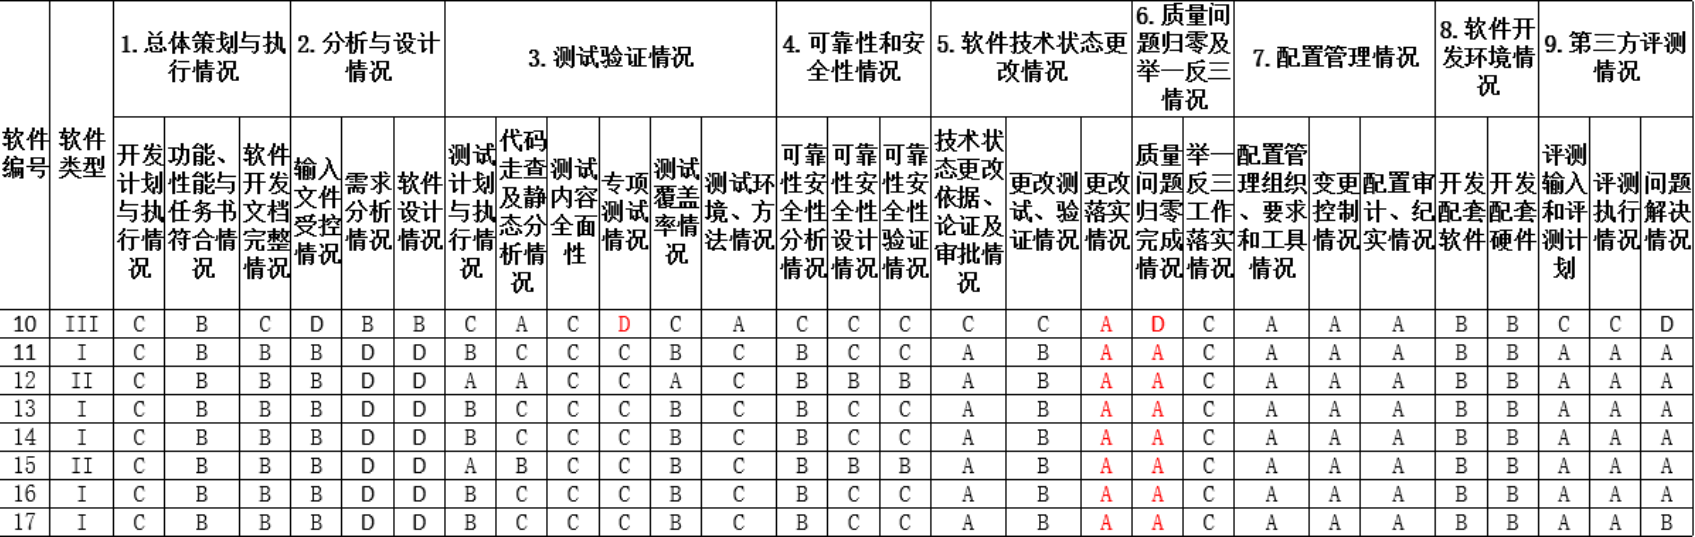
\includegraphics[width=0.8\textwidth]{img7/data.png}
\end{figure}

\subsection{度量元量化}

首先按照度量元的等级评价来进行数据量化,即:

\begin{itemize}
	\item 若度量元等级评价为A,则该度量元值$index=1$;类似地,若为B,则$index=0.9$;
	\item 若为C,则$index=0.7$;若为D,则$index =0.2$.
\end{itemize}

10 - 17 的量化后表格如下所示:

\begin{lstlisting} [language=Python, title=度量元等级评价量化]
scores = np.array([
    [7, 9, 7, 2, 9, 9, 7 , 10, 7, 2, 7 , 10, 7, 7, 7, 7 , 7, 10, 2 , 7, 10, 10, 10, 9, 9, 7 , 7 , 2 ],
    [7, 9, 9, 9, 2, 2, 9 , 7 , 7, 7, 9 , 7 , 9, 7, 7, 10, 9, 10, 10, 7, 10, 10, 10, 9, 9, 10, 10, 10],
    [7, 9, 9, 9, 2, 2, 10, 10, 7, 7, 10, 7 , 9, 9, 9, 10, 9, 10, 10, 7, 10, 10, 10, 9, 9, 10, 10, 10],
    [7, 9, 9, 9, 2, 2, 9 , 7 , 7, 7, 9 , 7 , 9, 7, 7, 10, 9, 10, 10, 7, 10, 10, 10, 9, 9, 10, 10, 10],
    [7, 9, 9, 9, 2, 2, 9 , 7 , 7, 7, 9 , 7 , 9, 7, 7, 10, 9, 10, 10, 7, 10, 10, 10, 9, 9, 10, 10, 10],
    [7, 9, 9, 9, 2, 2, 10, 9 , 7, 7, 9 , 7 , 9, 9, 9, 10, 9, 10, 10, 7, 10, 10, 10, 9, 9, 10, 10, 10],
    [7, 9, 9, 9, 2, 2, 9 , 7 , 7, 7, 9 , 7 , 9, 7, 7, 10, 9, 10, 10, 7, 10, 10, 10, 9, 9, 10, 10, 10],
    [7, 9, 9, 9, 2, 2, 9 , 7 , 7, 7, 9 , 7 , 9, 7, 7, 10, 9, 10, 10, 7, 10, 10, 10, 9, 9, 10, 10, 9 ]
])
\end{lstlisting}

\begin{figure}[H]
	\centering
	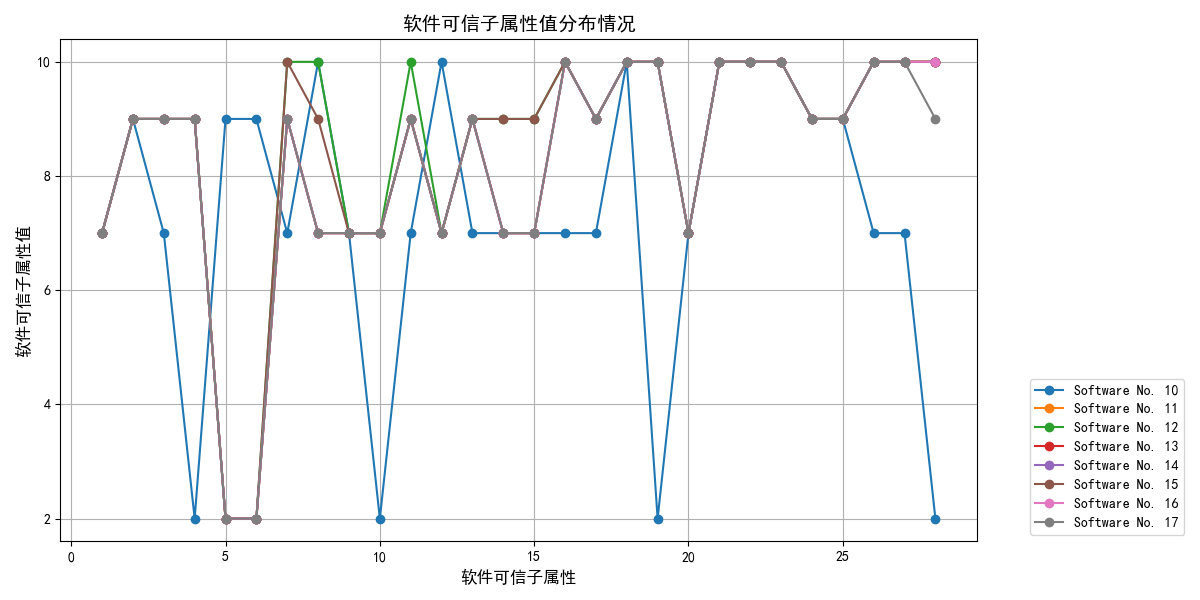
\includegraphics[width=0.7\textwidth]{img7/plt2.png}
	\caption{度量元等级评价分布情况折线图}	
\end{figure}


\subsection{子属性分组}

根据示例,每一个子属性下应该进行幂积运算,我们将子属性进行分组:

\begin{lstlisting} [language=Python, title=子属性分组]
# 子属性权重
sub_attribute_weights = np.array([
    0.31, 0.36, 0.33, # 总体策划与执行情况
    0.33, 0.33, 0.34, # 分析与设计情况
    0.16, 0.17, 0.17, 0.17, 0.17, 0.16, # 测试验证情况
    0.33, 0.34, 0.33, # 可靠性和安全性情况
    0.34, 0.33, 0.33, # 软件技术状态更改情况
    0.50, 0.50,       # 质量问题归零及举一反三情况
    0.33, 0.34, 0.33, # 配置管理情况
    0.50, 0.50,       # 软件开发环境情况
    0.33, 0.33, 0.34  # 第三方评测情况
])

lengths = [3, 3, 6, 3, 3, 2, 3, 2, 3]
results = []
\end{lstlisting}

下面,进行子属性的权重幂积运算:

\begin{lstlisting} [language=Python, title=子属性权重幂积运算]
	for row in scores:
		idx = 0
		row_results = []
		# 遍历每个组
		for length in lengths:
			x_i = row[idx:idx+length]
			w_i = sub_attribute_weights[idx:idx+length]
			G = np.prod(x_i ** w_i)
			row_results.append(G)
			idx += length  # 移动到下一个组
		results.append(row_results)
	
	results = np.array(results)
\end{lstlisting}

运算结果如下所示:

\begin{figure}[H]
	\centering
	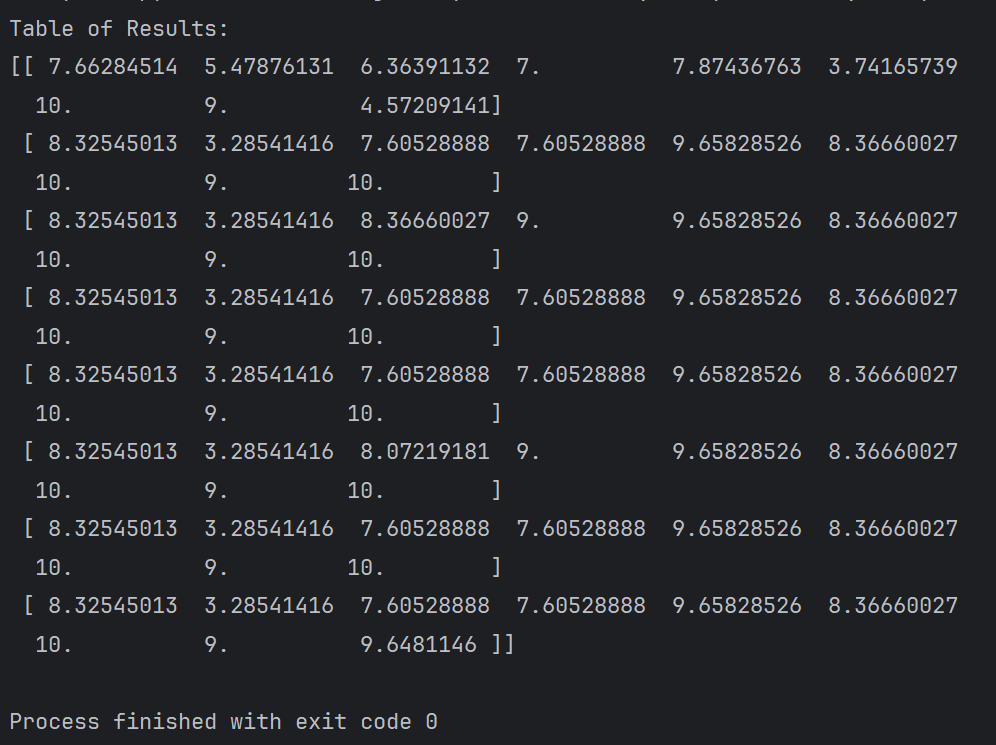
\includegraphics[width=0.4\textwidth]{img7/result1.png}
\end{figure}

\begin{table}[H]
	\centering
	\begin{tabular}{c|ccccccccc}
	\toprule
	\textbf{Row Index} &\textbf{1} & \textbf{2} & \textbf{Group 3} & \textbf{Group 4} & \textbf{Group 5} & \textbf{Group 6} & \textbf{Group 7} & \textbf{Group 8} & \textbf{Group 9} \\
	\midrule
	10 & 7.6628 & 5.4788 & 6.3639 & 7.0000 & 7.8744 & 3.7417 & 10.0000 & 9.0000 & 4.5721 \\
	11 & 8.3255 & 3.2854 & 7.6053 & 7.6053 & 9.6583 & 8.3666 & 10.0000 & 9.0000 & 10.0000 \\
	12 & 8.3255 & 3.2854 & 8.3666 & 9.0000 & 9.6583 & 8.3666 & 10.0000 & 9.0000 & 10.0000 \\
	13 & 8.3255 & 3.2854 & 7.6053 & 7.6053 & 9.6583 & 8.3666 & 10.0000 & 9.0000 & 10.0000 \\
	14 & 8.3255 & 3.2854 & 7.6053 & 7.6053 & 9.6583 & 8.3666 & 10.0000 & 9.0000 & 10.0000 \\
	15 & 8.3255 & 3.2854 & 8.0722 & 9.0000 & 9.6583 & 8.3666 & 10.0000 & 9.0000 & 10.0000 \\
	16 & 8.3255 & 3.2854 & 7.6053 & 7.6053 & 9.6583 & 8.3666 & 10.0000 & 9.0000 & 10.0000 \\
	17 & 8.3255 & 3.2854 & 7.6053 & 7.6053 & 9.6583 & 8.3666 & 10.0000 & 9.0000 & 9.6481 \\
	\bottomrule
	\end{tabular}
	\caption{结果表}
\end{table}

\begin{figure}[H]
	\centering
	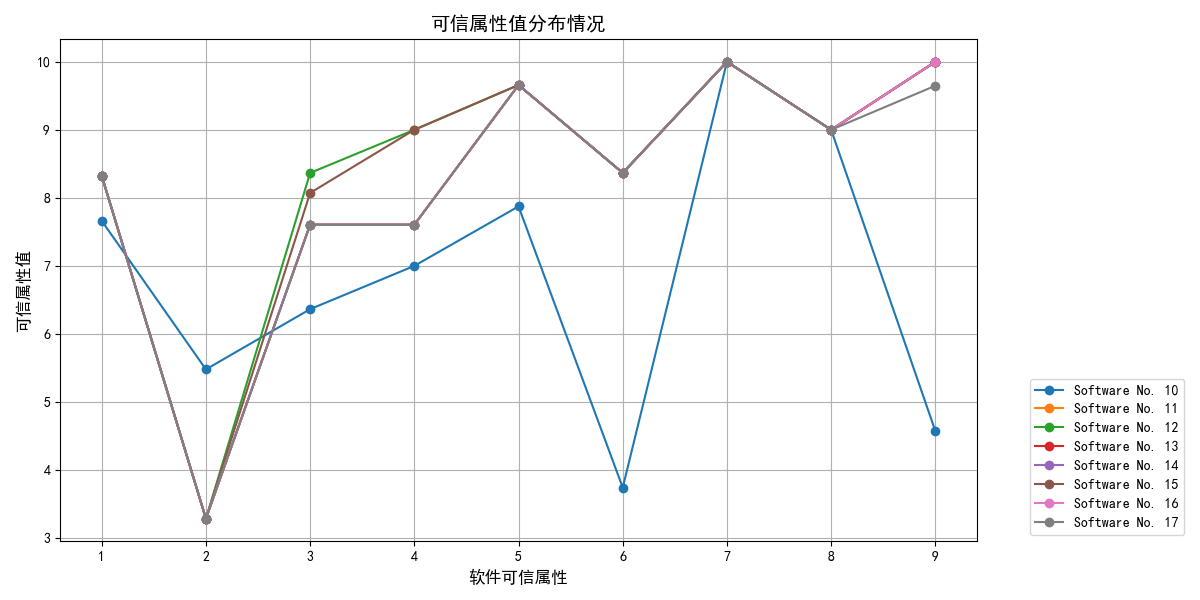
\includegraphics[width=0.7\textwidth]{img7/plt1.png}
	\caption{可信属性值分布情况折线图}	
\end{figure}

\subsection{软件可信度量值计算}

获得了输出的数据以后,接下来我们要对新的数据进行新的加权:

\begin{lstlisting} [language=Python, title=属性计算]
attribute_weights = np.array([0.05, 0.17, 0.20, 0.15, 0.09, 0.09, 0.11, 0.05, 0.09])

final_results = []
for row in results:
    # 幂积公式:x1^w1 * x2^w2 * ... * xn^wn
    final_value = np.prod(row ** attribute_weights)
    final_results.append(final_value)

final_results = np.array(final_results)
\end{lstlisting}

\begin{figure}[H]
	\centering
	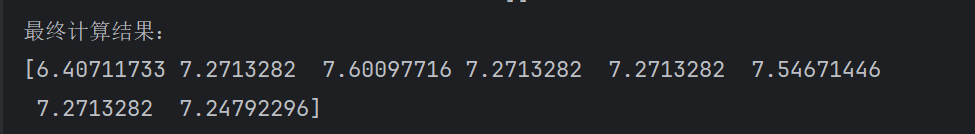
\includegraphics[width=0.5\textwidth]{img7/finalresult.png}
\end{figure}

结果表格如下:

\begin{table}[H]
	\centering
	\begin{tabular}{cc}
	\toprule
	\textbf{Row Index} & \textbf{Final Result} \\
	\midrule
	10 & 6.4071 \\
	11 & 7.2713 \\
	12 & 7.6010 \\
	13 & 7.2713 \\
	14 & 7.2713 \\
	15 & 7.5467 \\
	16 & 7.2713 \\
	17 & 7.2479 \\
	\bottomrule
	\end{tabular}
	\caption{最终计算结果表}
\end{table}

\subsection{分级计算}

\begin{figure}[H]
	\centering
	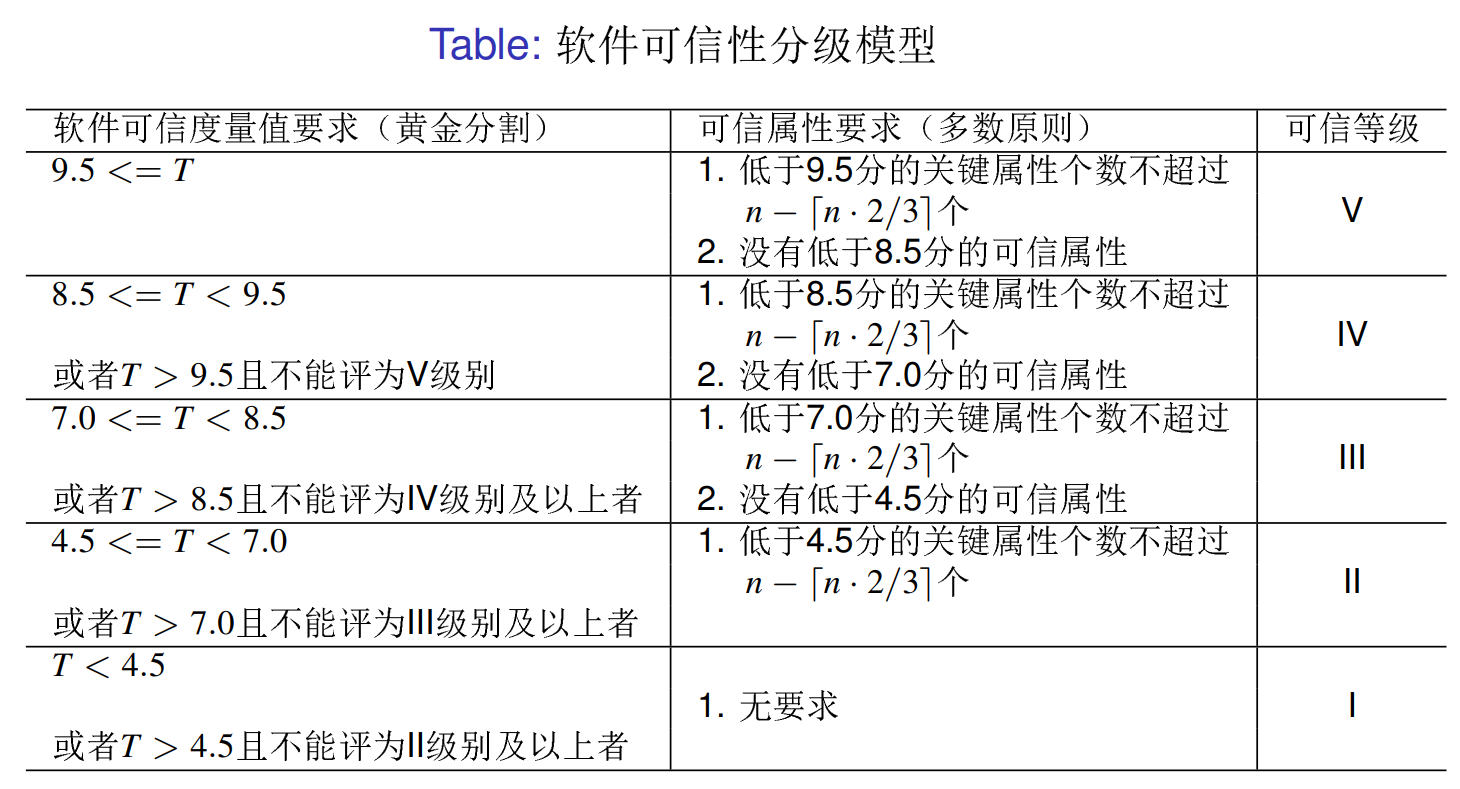
\includegraphics[width=0.5\textwidth]{img7/levels.png}
	\caption{软件可信度等级判定方法}
\end{figure}

根据上述标准,我们可以写出相关的代码:

\begin{lstlisting} [language=Python, title=分级计算]
	def classify_trust_levels(final_results, attribute_scores):
    trust_levels = []
    for T, scores in zip(final_results, attribute_scores):
        n = len(scores)
        print(f"n的个数为{n}")
        threshold_2_3 = n - int(np.ceil(2 * n / 3)) # 使用 ceil 函数向上取整
        print(f"不能超过{threshold_2_3}个")

        # 统计低于某些阈值的属性个数
        low_9_5 = np.sum(scores < 9.5)
        low_8_5 = np.sum(scores < 8.5)
        low_7_0 = np.sum(scores < 7.0)
        low_4_5 = np.sum(scores < 4.5)

        if T >= 9.5 and low_9_5 <= threshold_2_3 and low_8_5 == 0:
            trust_levels.append("V")
            continue

        if (8.5 <= T < 9.5 and low_8_5 <= threshold_2_3 and low_7_0 == 0) or (T > 9.5 and "V" not in trust_levels):
            trust_levels.append("IV")
            continue

        if (7.0 <= T < 8.5 and low_7_0 <= threshold_2_3 and low_4_5 == 0) or (T > 8.5 and "IV" not in trust_levels):
            trust_levels.append("III")
            continue

        if (4.5 <= T < 7.0 and low_4_5 <= threshold_2_3) or (T > 7.0 and "III" not in trust_levels):
            trust_levels.append("II")
            continue

        if T < 4.5 or (T > 4.5 and "II" not in trust_levels):
            trust_levels.append("I")
            continue

    return trust_levels

# 计算可信等级
trust_levels = classify_trust_levels(final_results, results)
print(trust_levels)
\end{lstlisting}

\begin{figure}[H]
	\centering
	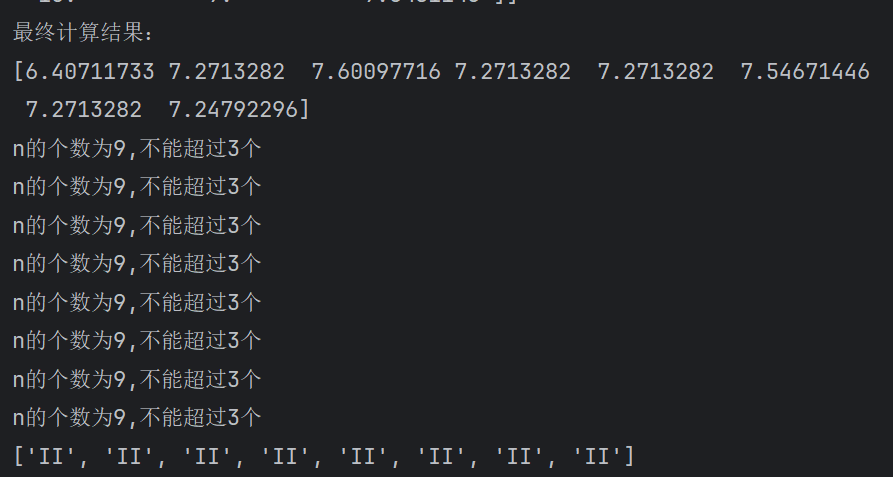
\includegraphics[width=0.5\textwidth]{img7/level.png}
	\caption{软件可信度等级判定结果}
\end{figure}

\subsection{总结}

最终的计算结果表格应如下所示:

\begin{table}[H]
	\centering
	\begin{tabular}{c|ccccccccc|c|c}
	\toprule
	\textbf{Index} &\textbf{1} & \textbf{2} & \textbf{3} & \textbf{4} & \textbf{5} & \textbf{6} & \textbf{7} & \textbf{8} & \textbf{9} & \textbf{Value} & \textbf{Level} \\
	\midrule
	10 & 7.6628 & 5.4788 & 6.3639 & 7.0000 & 7.8744 & 3.7417 & 10.0000 & 9.0000 & 4.5721  & 6.4071 & II \\
	11 & 8.3255 & 3.2854 & 7.6053 & 7.6053 & 9.6583 & 8.3666 & 10.0000 & 9.0000 & 10.0000 & 7.2713 & II \\
	12 & 8.3255 & 3.2854 & 8.3666 & 9.0000 & 9.6583 & 8.3666 & 10.0000 & 9.0000 & 10.0000 & 7.6010 & II \\
	13 & 8.3255 & 3.2854 & 7.6053 & 7.6053 & 9.6583 & 8.3666 & 10.0000 & 9.0000 & 10.0000 & 7.2713 & II \\
	14 & 8.3255 & 3.2854 & 7.6053 & 7.6053 & 9.6583 & 8.3666 & 10.0000 & 9.0000 & 10.0000 & 7.2713 & II \\
	15 & 8.3255 & 3.2854 & 8.0722 & 9.0000 & 9.6583 & 8.3666 & 10.0000 & 9.0000 & 10.0000 & 7.5467 & II \\
	16 & 8.3255 & 3.2854 & 7.6053 & 7.6053 & 9.6583 & 8.3666 & 10.0000 & 9.0000 & 10.0000 & 7.2713 & II \\
	17 & 8.3255 & 3.2854 & 7.6053 & 7.6053 & 9.6583 & 8.3666 & 10.0000 & 9.0000 & 9.6481  & 7.2479 & II \\
	\bottomrule
	\end{tabular}
	\caption{结果表}
\end{table}



\end{document}